% !TeX encoding = UTF-8
% !TeX root = master.tex
% !TeX spellcheck = en_US

\documentclass[10pt,final,conference,letterpaper,oneside,twocolumn]{styles/IEEEtran}

\usepackage[utf8]{inputenc}
\usepackage[english]{babel}
\selectlanguage{english}
\usepackage{graphicx}
\usepackage{grffile}
\graphicspath{{figures/}}
\usepackage{float}
\usepackage{booktabs}
\usepackage{tabu}
\usepackage{rotating}
\usepackage{array}
\usepackage{multirow}
\usepackage{url}
\usepackage{footnote}
\usepackage{footmisc}
\usepackage[nonumberlist,acronym,xindy]{glossaries}
\usepackage{cooltooltips}
\usepackage{mathtools}
\usepackage[noabbrev,nameinlink]{cleveref}

\ifCLASSOPTIONcompsoc
\usepackage[nocompress]{cite}
\else
\usepackage{cite}
\fi

\ifCLASSOPTIONcompsoc
\usepackage[caption=false,font=normalsize,labelfont=sf,textfont=sf]{subfig}
\else
\usepackage[caption=false,font=footnotesize]{subfig}
\fi

\makeglossaries

% abbreviations:
\newacronym{cad}{CAD}{Computer Aided Design}
\newacronym{ner}{NER}{Named Entity Recognition}



\begin{document}



%---------------------------------------------------------------------------------------------------
% Top matter
%---------------------------------------------------------------------------------------------------

\title{Dataset for extraction of assembly information from instruction manuals}

\author{\IEEEauthorblockN{Carlos M. Costa}
	\IEEEauthorblockA{Faculty of Engineering\\
		University of Porto\\
		Rua Dr. Roberto Frias, s/n 4200-465, Porto, Portugal\\
		Email: carlos.costa@fe.up.pt
	}
}

\IEEEtitleabstractindextext{%
	\begin{abstract}

Teaching industrial robots by demonstration can significantly decrease the re-purposing costs of assembly lines worldwide. To achieve this goal, the robot needs to semantically detect and track each object component with high accuracy. To speedup the object recognition phase, the learning system can gather information from assembly manuals in order to identify which objects are required for assembling the new product and if possible also extract the assembly order and spatial relation between them. This paper presents a dataset to test a \gls{ner} system with these goals. The dataset contains assembly operations for alternators, gearboxes and engines, which were written in a language discourse that ranges from professional to informal. For validating a given \gls{ner} system with this dataset, each assembly operation has a list of the named entities and the required quantities for performing the product assembly. This allows to evaluate \gls{ner} systems using precision, recall, accuracy and F1 scores. The dataset can also be used to evaluate information extraction and computer vision systems, since most assembly operations have pictures of the objects to assemble and also diagrams showing the necessary product parts, their assembly order and spacial disposition.

\end{abstract}

	\begin{IEEEkeywords}
		Natural Language Processing Dataset, Named Entity Recognition, Small Parts Assembly, Industrial Robotics
	\end{IEEEkeywords}
}

\maketitle
\IEEEdisplaynontitleabstractindextext


%---------------------------------------------------------------------------------------------------
% Sections
%---------------------------------------------------------------------------------------------------

\section{Introduction}\label{sec:introduction}

Programming of industrial robots for assembly operations is a meticulous and arduous task that requires a significant engineering effort and long testing and deployment phases. For high volume manufacturing this cost is acceptable, but it is too expensive to repurpose robots for small volume production using traditional programming approaches. These issues can be overcome with robots that can learn new assembly skills by observing experienced operators and interacting with them through natural language. To achieve these goals, the robot needs to successfully recognize the objects within its workspace and semantically track their pose with high precision while the operator demonstrates how to perform the assembly operations. Moreover, it must be able to understand any instructions that the operator might give and also have the ability to recall them if asked later on. This type of teaching allows rapid reprogramming of flexible robotic assembly cells for new tasks. This process can be speed up further if there are assembly manuals available, which allows the robotic system to extract the objects and their assembly spacial disposition from the textual and visual representations. By knowing which objects to expect for a given teaching session, the object recognition efficiency can be significantly increased (by limiting the object search database). Moreover, this preliminary information extraction phase reduces the human teaching phase to only the operations that lack detailed information.

This paper presents a dataset for evaluating \gls{ner} systems.

\section{Related work}\label{sec:related-work}

\gls{nlp} algorithms have been integrated into robotics systems for a myriad of applications, ranging from control of industrial robotic arms \cite{Akan2011,Watanabe2006} and mobile robots \cite{Matuszek2013} to complex interaction with humanoid systems using a combination of voice, text and image perception analysis \cite{Neo2008,Barabas2012}. For the voice and textual teaching, the objects names and relations can be identified using \gls{ner} algorithms \cite{Leon2014,Dlugolinsky2013}. This type of approach usually relies on syntactic and semantic parsing of the text and also in machine learning algorithms \cite{Ekbal2012} in order to be able to recognize previously unseen object names. It may present some challenges \cite{Ratinov2009}, but this methodology can achieve multilingual entity recognition \cite{Rami2014} if language agnostic attributes are used.

Advanced applications of \gls{nlp} algorithms include the teaching of assembly operations to robot arm manipulation systems by human operators. The JAST robot presented in \cite{Rickert2007} was implemented using a multi-agent system capable of learning assembly operations by interpreting human voice commands along with their gestures and gaze. The speech recognition system uses a \gls{ccg} and a semantics module to analyze if the operator is making statements for teaching, asking for information or giving answers to previous questions made by the robot. The vision system besides tracking the hands and gaze of the operator to perform a better speech analysis, it also recognizes the assembly objects within the robot workspace using template matching techniques.

Another example of usage of \gls{nlp} methods in an industrial scenario is presented in \cite{Stenmark2013}, in which it is used a multi-lingual statistical semantic parser to extract assembly operations from natural language sentences given by remote operators. The system was developed using a client-server architecture, containing a natural language parser, a \gls{kif} and an engineering system. The parser finds predicates with their respective arguments in sentences and establishes coreference chains. The \gls{kif} contains ontologies and semantically annotated skills that are used for filtering the predicates and return only the ones relevant for assembly operations. Lastly, the engineering system is a high level programming interface that uses the predicates found by the parser to select the appropriate skills for assembly while also matching the predicates arguments with the knowledge database in order to identify the objects and analyze in which branch of the assembly tree they must be inserted for achieving proper assembly order.

Besides voice and textual input from humans, the assembly information can also be retrieved from online web pages or knowledge repositories. The system proposed in \cite{Tenorth2010} can extract the assembly graph by performing a syntactic and semantic analysis using a \gls{pcfg} parser and a \gls{pos} tagger followed by word sense retrieval and disambiguation using the WordNet database and the Cyc ontology. After having a preliminary assembly plan, it is executed in simulation to perform a high level validation and also to allow the optimization of the robot movements. If ambiguous or missing information is detected, the system tries to generate a valid assembly plan by analyzing the objects' environment, assembly context and also similar operations stored in its knowledge base.

Named entity recognition can also be useful to identify key information from mission operation orders given to operators of robotics systems, such as \glspl{uav}. Highlighting entities such as persons, times, locations, coordinates, targets and organizations allows the human operators to extract the necessary mission information faster. Moreover, in the future it might even be possible to have the robotic system autonomously extract all the required information to carry on the mission without human assistance. The system introduced in \cite{Chesworth2016} was the first step towards this goal, and it was able to extract named entities from textual documents using \glspl{crf} statistical models that relied on features such as word lists, regular expressions, prefixes / sufixes, word case and also unigram / bigram / trigrams models. The evaluation of the \gls{ner} system was performed using metrics such as precision, recall and accuracy and used 9-fold cross validation for having a rotating train / test dataset in order to avoid model over-fitting.

Several datasets for \gls{ner} have been presented over the years for news and tweets \cite{Dojchinovski2013,Roder2014}. This paper aims to provide a dataset for evaluating \gls{ner} systems with a corpus containing a diverse range of assembly operations for small complex objects (alternators, gearboxes and engines) written in a language discourse that ranges from professional to informal.

\section{Dataset sources}\label{sec:dataset-sources}

This dataset is composed of 10 English instruction manuals with 453 pages detailing assembly operations of alternators, engines and gearboxes. These object categories were selected because they have small, light and diverse components that a typical industrial robot arm can manipulate and also because they have increasing complexity (from the simple gearboxes to the much more complex fuel / steam engines). These manuals were selected for performing \gls{ner} because they are a representative sample of the several types of manuals that are available for operators working in small parts assembly and also because they were written with a language discourse ranging from very concise and professional to a more colloquial and unstructured type. Moreover they provide tables / lists with the parts and tools required for the assembly operations which are very useful for evaluating \gls{ner} systems.

Most of these assembly instruction manuals are single column (two of them are dual column) and have \gls{cad} drawings or pictures alongside the assembly procedures. Moreover, some of these procedures are very long, with the description of all the necessary parts for the entire assembly operation (in the case of the alternators), while others have the assembly operations split across the main object components.


\subsection{Alternators}

Alternators are electrical generators that convert mechanical energy into electric energy in the form of alternating current. Their assembly is quite complex, involving a lot of small parts and intricate wire bending.

This dataset includes the detailed assembly of two automotive alternators (used to power the electric equipment of cars and charge their battery). One of them was written in a dual column layout with a lot of diagrams and in a professional and concise language style while the other one was written in single column informal language discourse while using mostly pictures instead of technical diagrams.


\subsection{Gearboxes}

Gearboxes are mechanical transmission systems that provide speed and torque conversions while also giving the option of forward and backwards wheel movement. They allow a typical car engine that operates at [600, 7000] \gls{rpm} to move the wheels with high torque when using lower gears and with high speed when employing higher gears. They give the user a high level of control over the engine performance allowing better fuel efficient and reducing engine wear.




\subsection{Engines}

FF.



\begin{table*}[t]
	\caption{Dataset overview}
	\tabulinesep = 1.3ex
	\centering
	\begin{tabu} { X[2.5,m,c] | X[m,c] X[m,c] X[m,c] X[m,c] }
		\rowfont{\bfseries\itshape} 	& Alternators									& Engines																& Gearboxes 										& Global 	\\
		\hline
		Number of pages 				& \cooltooltip[1 1 1]{}{}{30+54}{}{84}			& \cooltooltip[1 1 1]{}{}{70+12+15+19+19+13}{}{148}						& \cooltooltip[1 1 1]{}{}{18+203}{}{221}			& 453		\\
		Number of assembly procedures 	& \cooltooltip[1 1 1]{}{}{1+1}{}{2}				& \cooltooltip[1 1 1]{}{}{35+1+1+1+1+1}{}{40}							& \cooltooltip[1 1 1]{}{}{1+52}{}{53}				& 95		\\
		Number of words					& \cooltooltip[1 1 1]{}{}{4009+5385}{}{9394}	& \cooltooltip[1 1 1]{}{}{9151+1851+1697+4063+4140+1993}{}{22895}		& \cooltooltip[1 1 1]{}{}{923+31169}{}{32092}		& 64381		\\
		Number of characters			& \cooltooltip[1 1 1]{}{}{25240+30941}{}{56181}	& \cooltooltip[1 1 1]{}{}{54386+10489+9451+22782+23138+11482}{}{131728}	& \cooltooltip[1 1 1]{}{}{6492+186083}{}{192575}	& 380484	\\
	\end{tabu}
	\label{tab:dataset-sources_dataset-overview}
\end{table*}

\section{Dataset preparation}\label{sec:dataset-preparation}

Automatic extraction of text from \gls{pdf} files with multi-column text, tables and large number of images and diagrams is a challenging task for any \gls{nlp} system. As such, the dataset preparation included the automatic extraction of text from the \gls{pdf} files, followed by a manual cleaning and inspection phase in which all the text that was not related to assembly operations was removed. To speedup this process and ensure proper text cleaning across the entire dataset, it was applied a set of regular expressions in order to remove page headers and footers and correct formating issues related with the text extraction. After this preprocessing stage, the dataset was proofread to correct spelling errors.

Later on the lists / tables with the information about the required assembly parts / tools was moved into validation files in order to allow the evaluation of a given \gls{ner} system.

Given that some \gls{nlp} toolkits such as the \gls{srilm} \cite{Stolcke2002} expect tokenized text when building N-gram models, a set of regular expressions was applied to the dataset in order to separate the words from the punctuation. Later on, the cleaned text extracted from the \glspl{pdf} was merged into training (75\%) and testing (25\%) files according to its respective category, namely the alternators, engines, gearboxes and the entire dataset. These merged files have two versions, one with the original cleaned text and another version with the tokenized text.

\section{N-grams language models}\label{sec:n-grams}

An n-gram is a contiguous sequence of items (typically letters or words) that are extracted from an information source (normally text, speech, images or \gls{dna}). By counting the n-grams in a knowledge corpus they can be used to create probabilistic language models for predicting the next item given a context. This is useful when developing speech recognizers and \gls{ocr} systems because the n-gram language model can help disambiguate items in the recognition process. Moreover they can be used for implementing text generators or suggestion / auto-complete systems and can also be applied to improve the efficiency of compression / search algorithms.



\subsection{Rank-frequency graphs}

Rank-frequency graphs are useful to analyze the word / n-gram diversity of a given text corpus. They are usually plotted in logarithmic scale and have the word rank in the X axis and the word frequency in the Y axis. They are also useful to check if a given text corpus follows the Zipf's law \cite{Piantadosi2014}, which states that the frequency of a given word in a text corpus is inversely proportional to its rank in the frequency table (as shown in \cref{eq:zipf-law}).

\begin{equation}\label{eq:zipf-law}
f(r) \propto \frac{1}{r^\alpha}
\end{equation}

Analyzing \crefrange{fig:rank-frequency-unigram}{fig:rank-frequency-pentagram} it can be seen that the dataset unigrams to pentagrams follow roughly the Zipf's law. Moreover, the alpha value introduced in \cref{eq:zipf-law} that best fits the plotted data starts at 0.25 in the first plot section, then increases to 0.5 in the middle plot section and becomes 1.0 in the last plot section. This is a typical behavior found in most languages \cite{NemethZainko2003}.

\begin{figure}[hb]
	\centering
	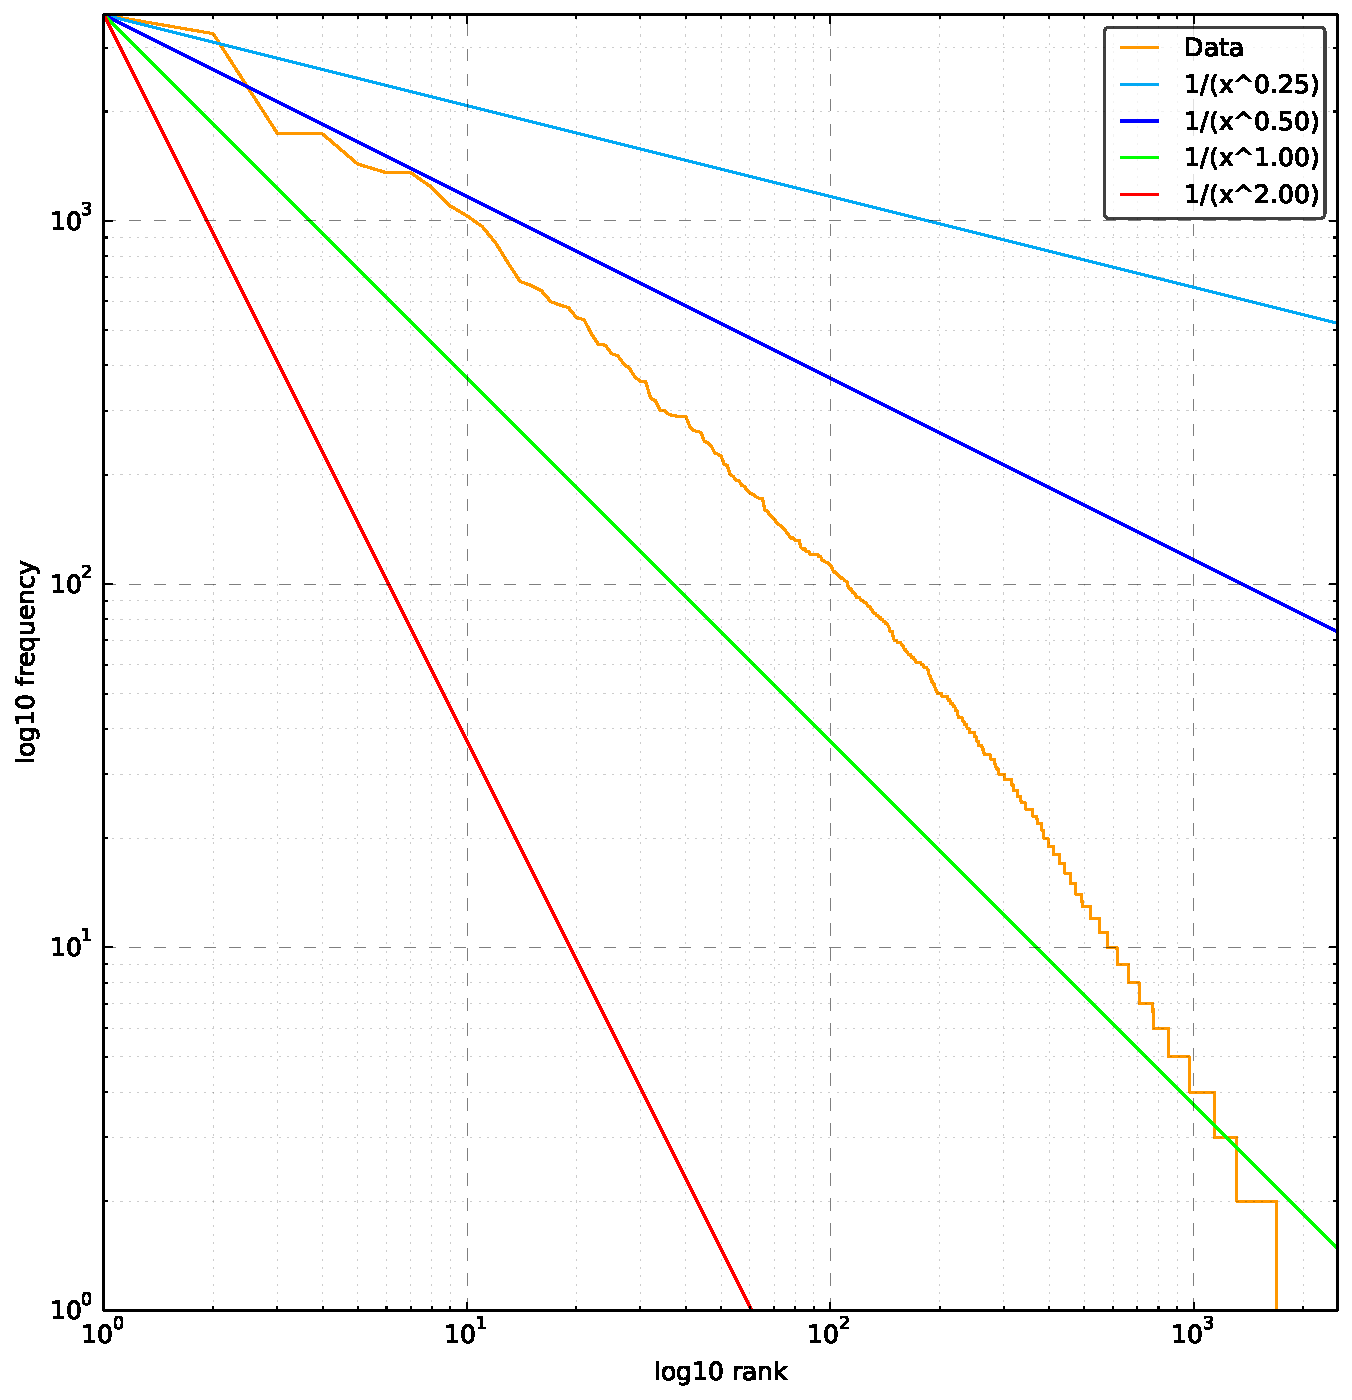
\includegraphics[width=0.9\linewidth]{figures/frequency-graphs/1-gram}
	\caption{Unigram rank-frequency graph of tokenized dataset}
	\label{fig:rank-frequency-unigram}
\end{figure}

\begin{figure}[ht]
	\centering
	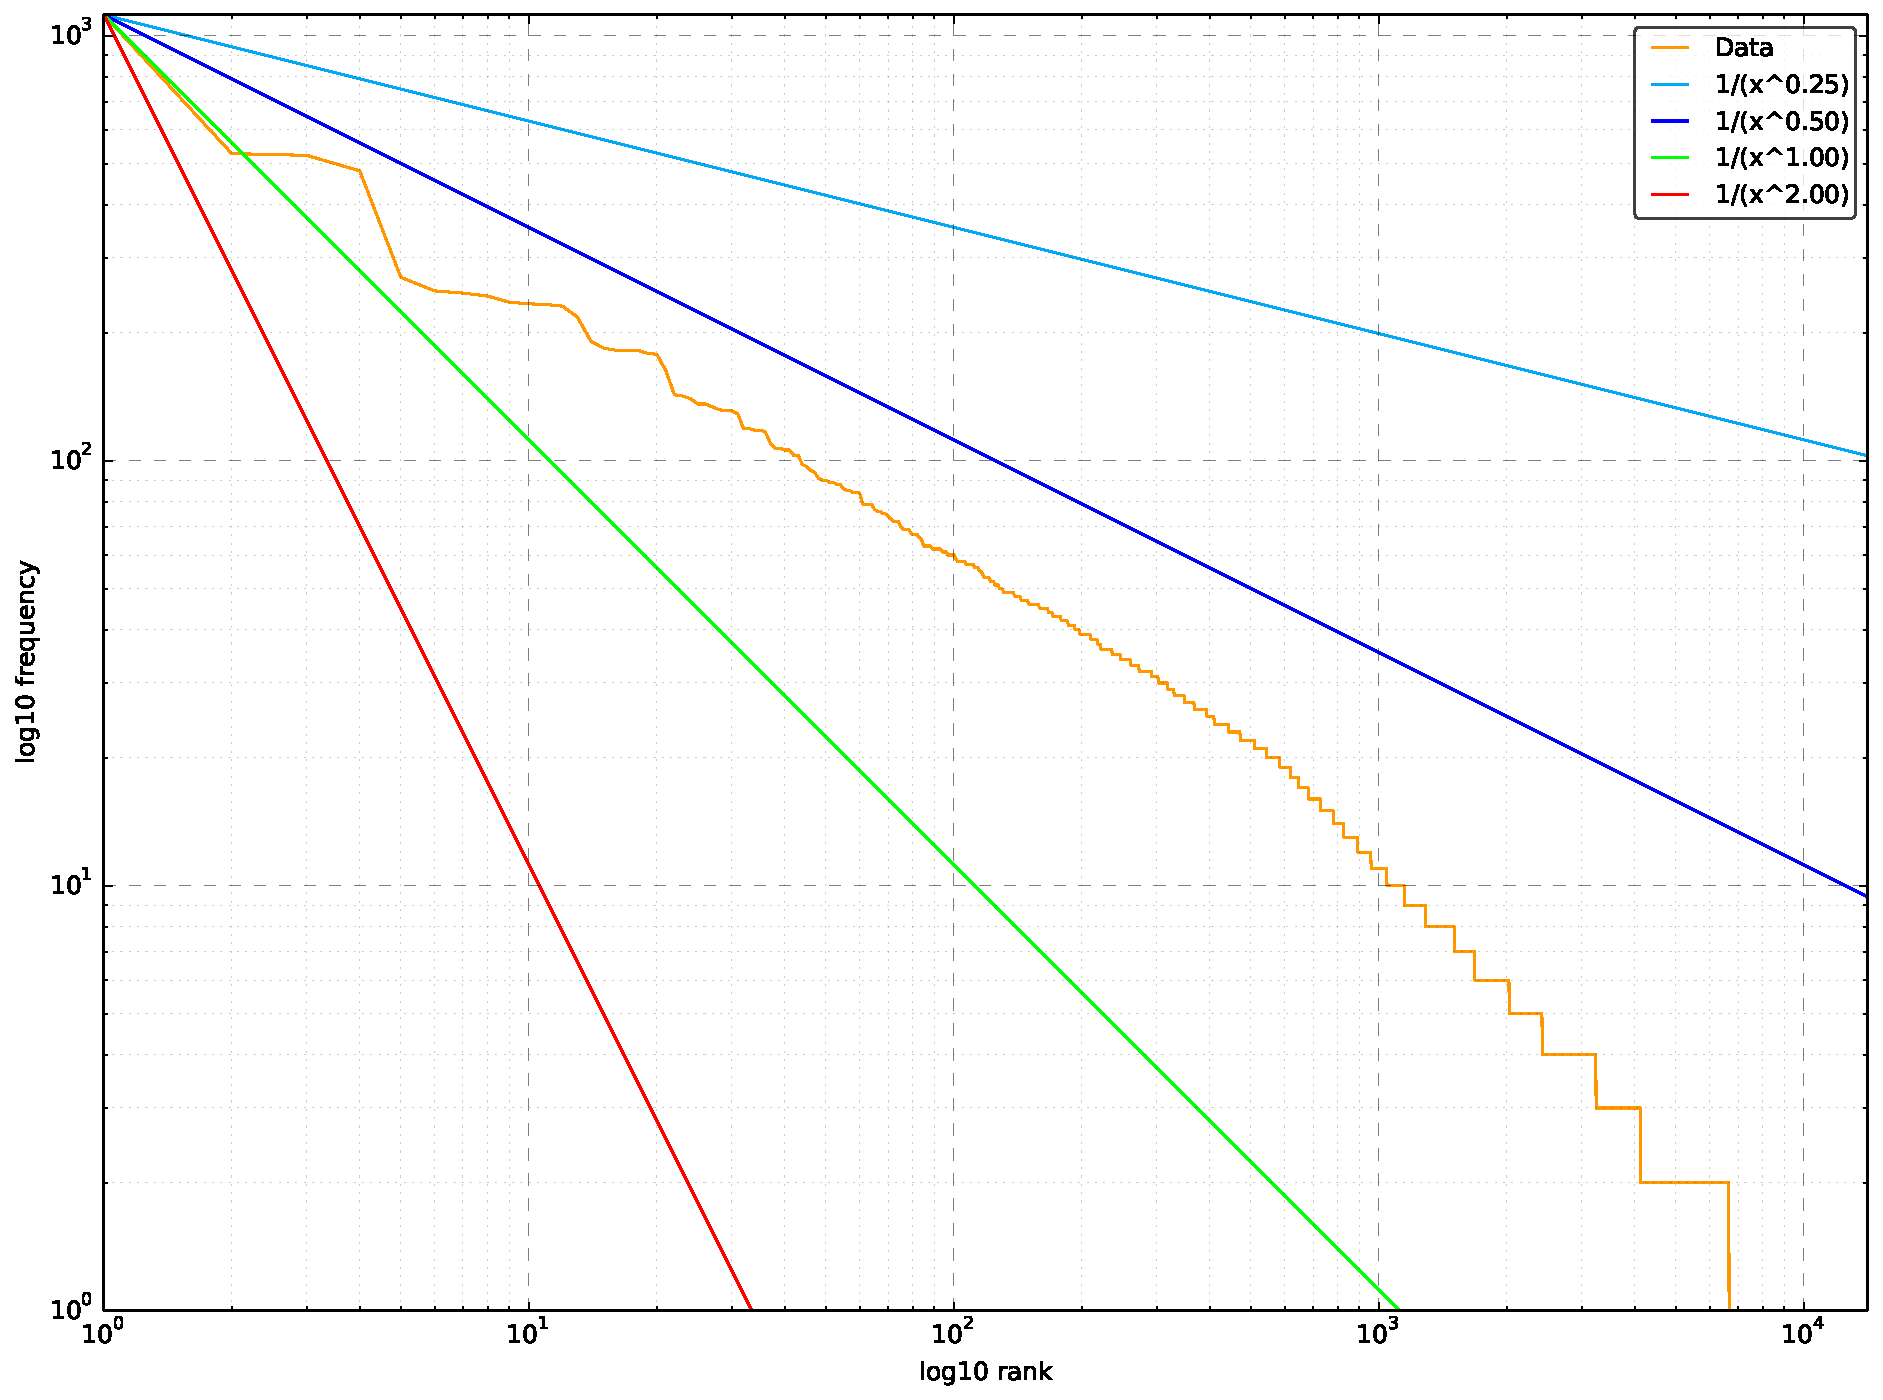
\includegraphics[width=0.9\linewidth]{figures/frequency-graphs/2-gram}
	\caption{Bigram rank-frequency graph of tokenized dataset}
	\label{fig:rank-frequency-bigram}
\end{figure}

\begin{figure}[ht]
	\centering
	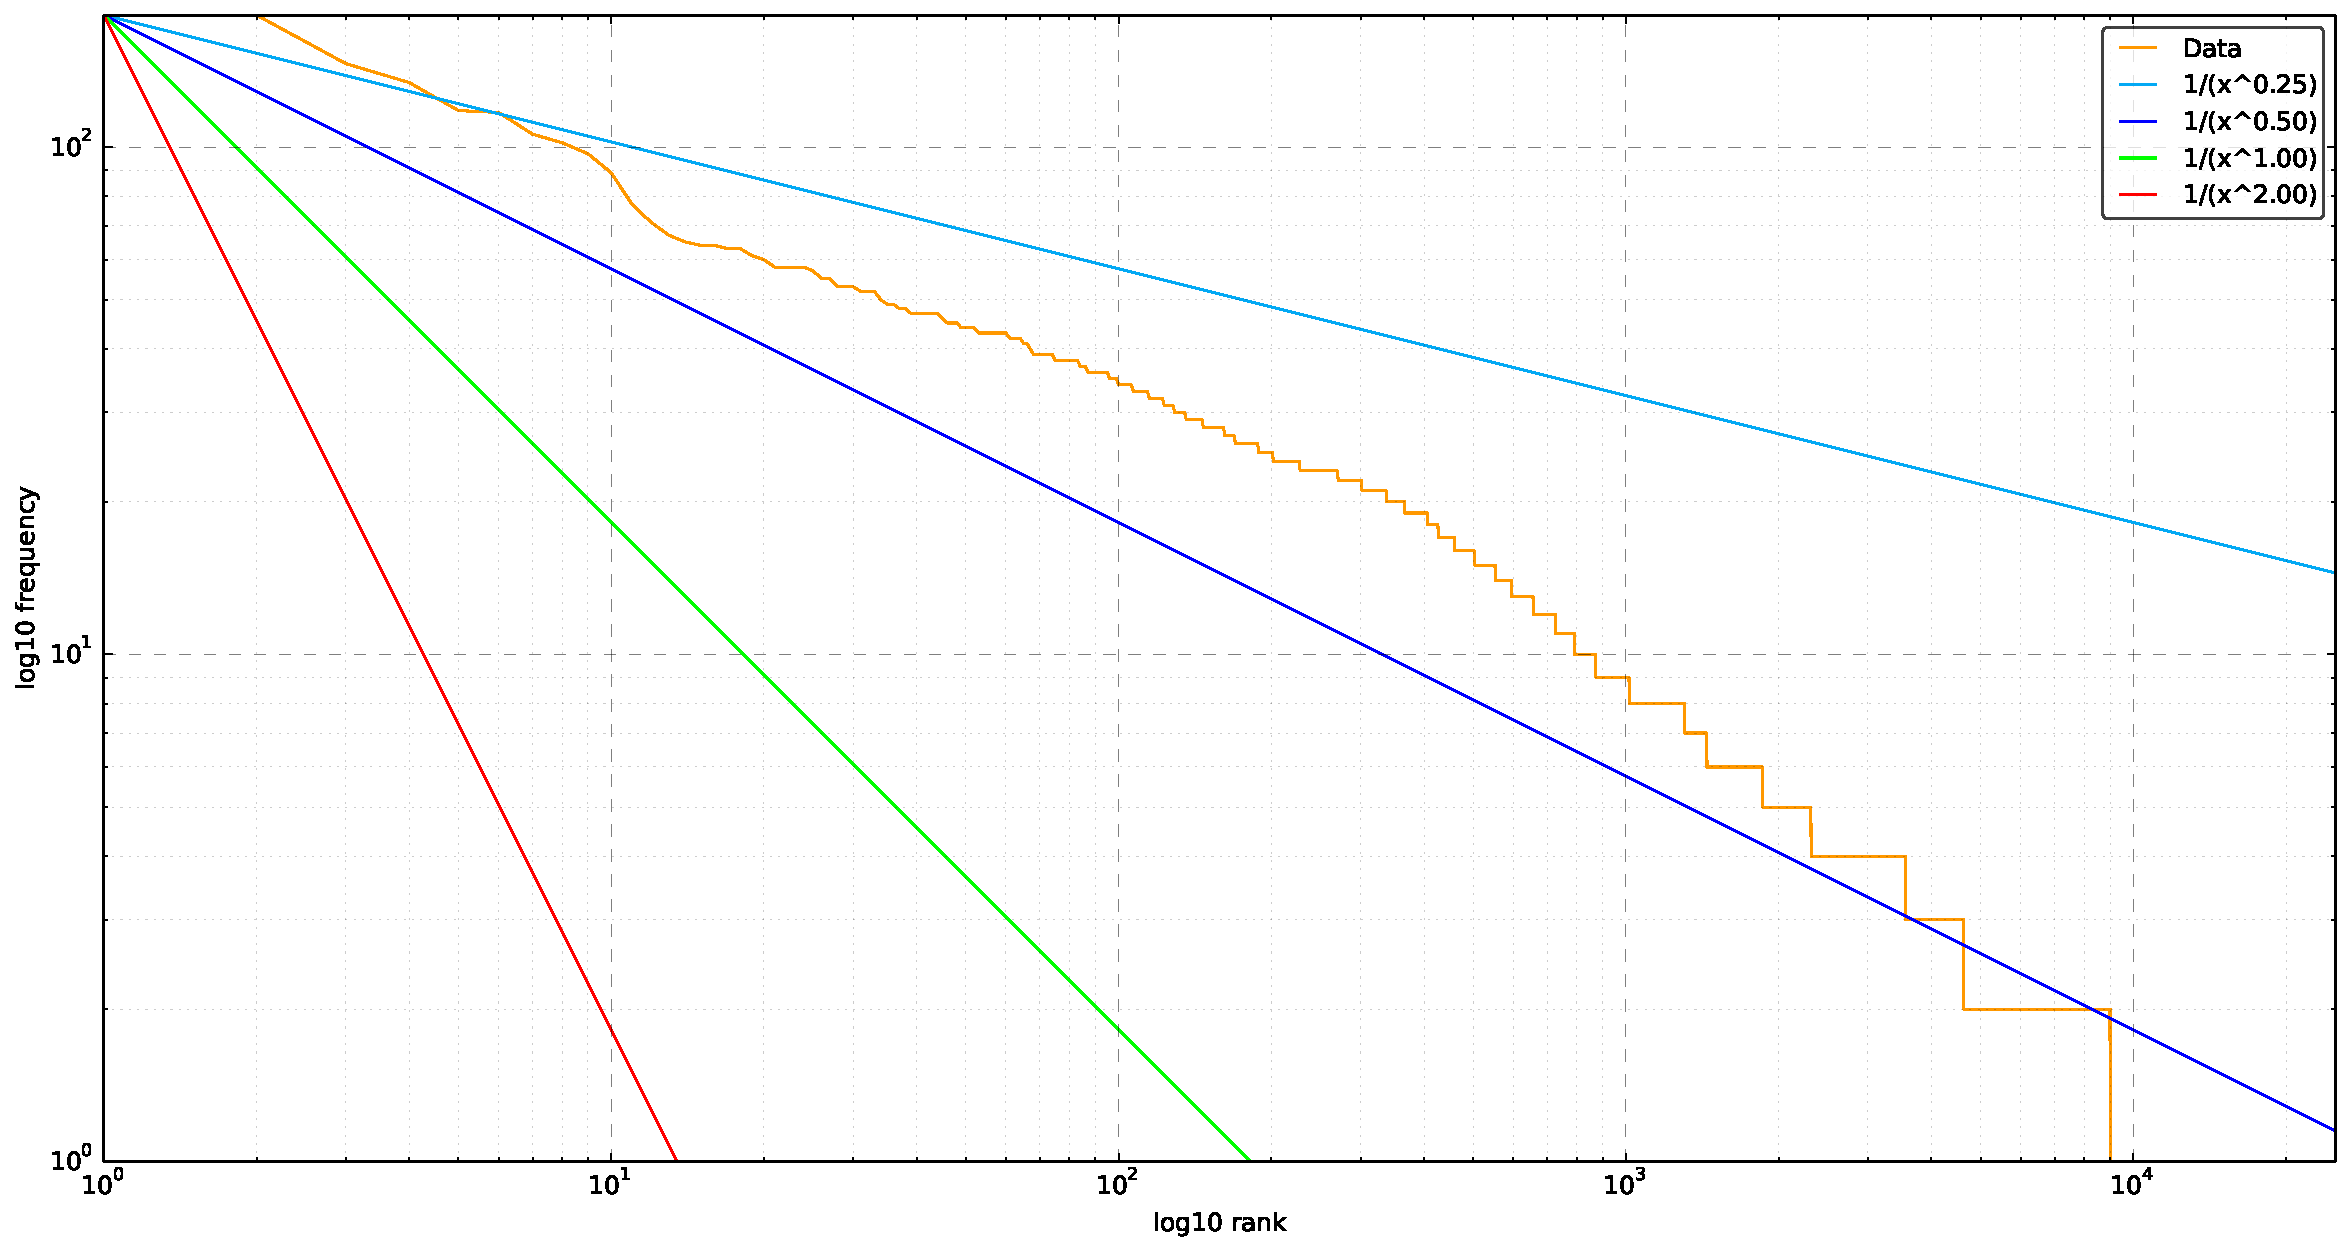
\includegraphics[width=0.9\linewidth]{figures/frequency-graphs/3-gram}
	\caption{Trigram rank-frequency graph of tokenized dataset}
	\label{fig:rank-frequency-trigram}
\end{figure}

\begin{figure}[ht]
	\centering
	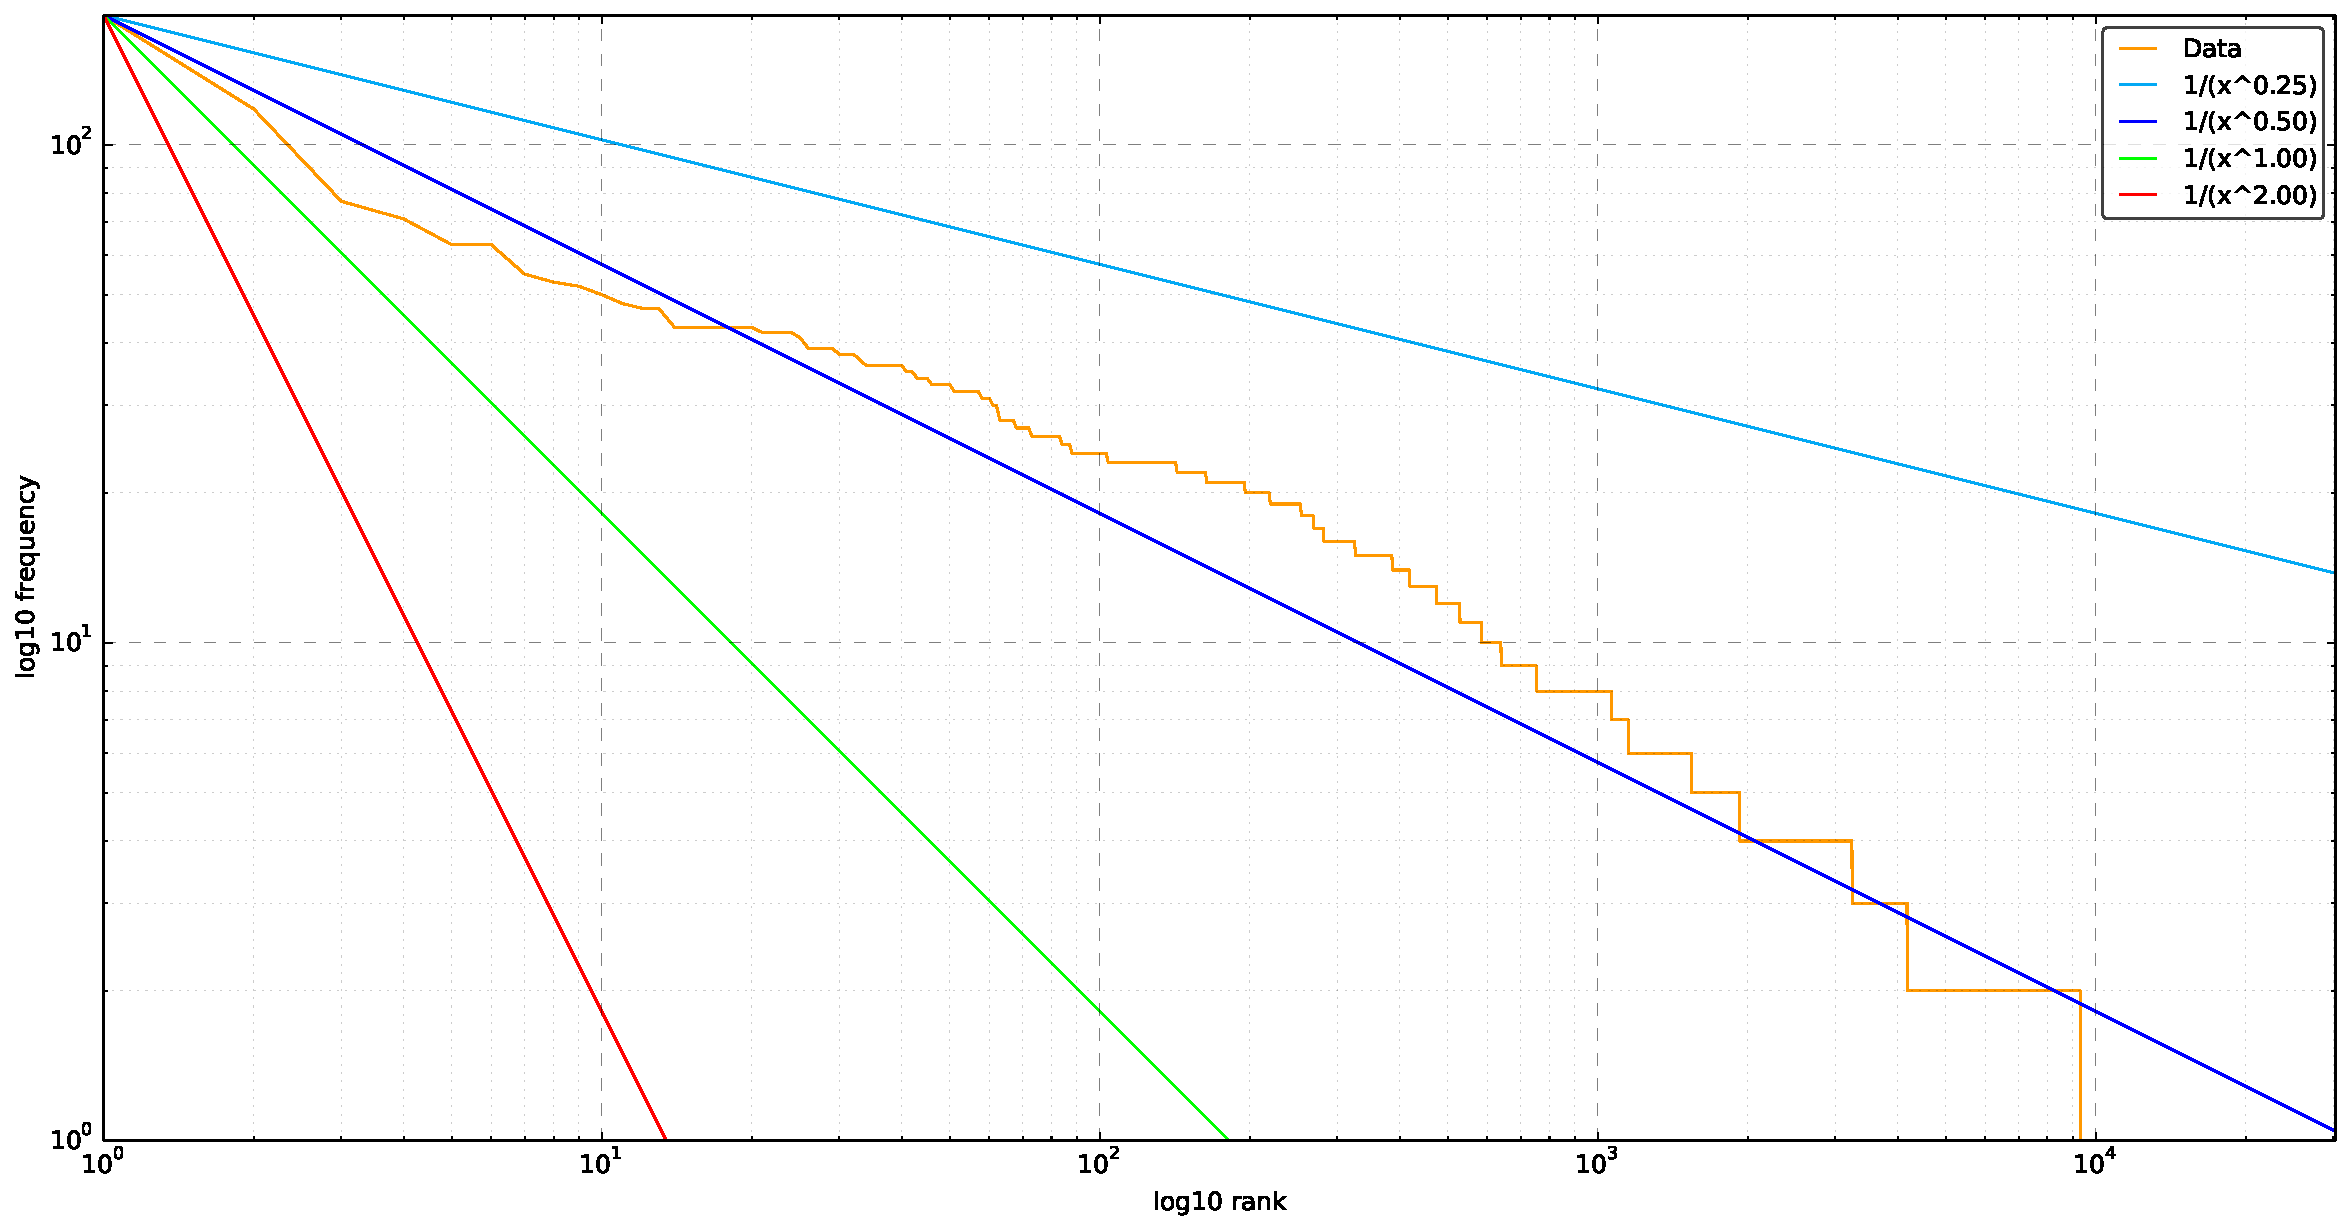
\includegraphics[width=0.9\linewidth]{figures/frequency-graphs/4-gram}
	\caption{Tetragram rank-frequency graph of tokenized dataset}
	\label{fig:rank-frequency-tetragram}
\end{figure}

\begin{figure}[ht]
	\centering
	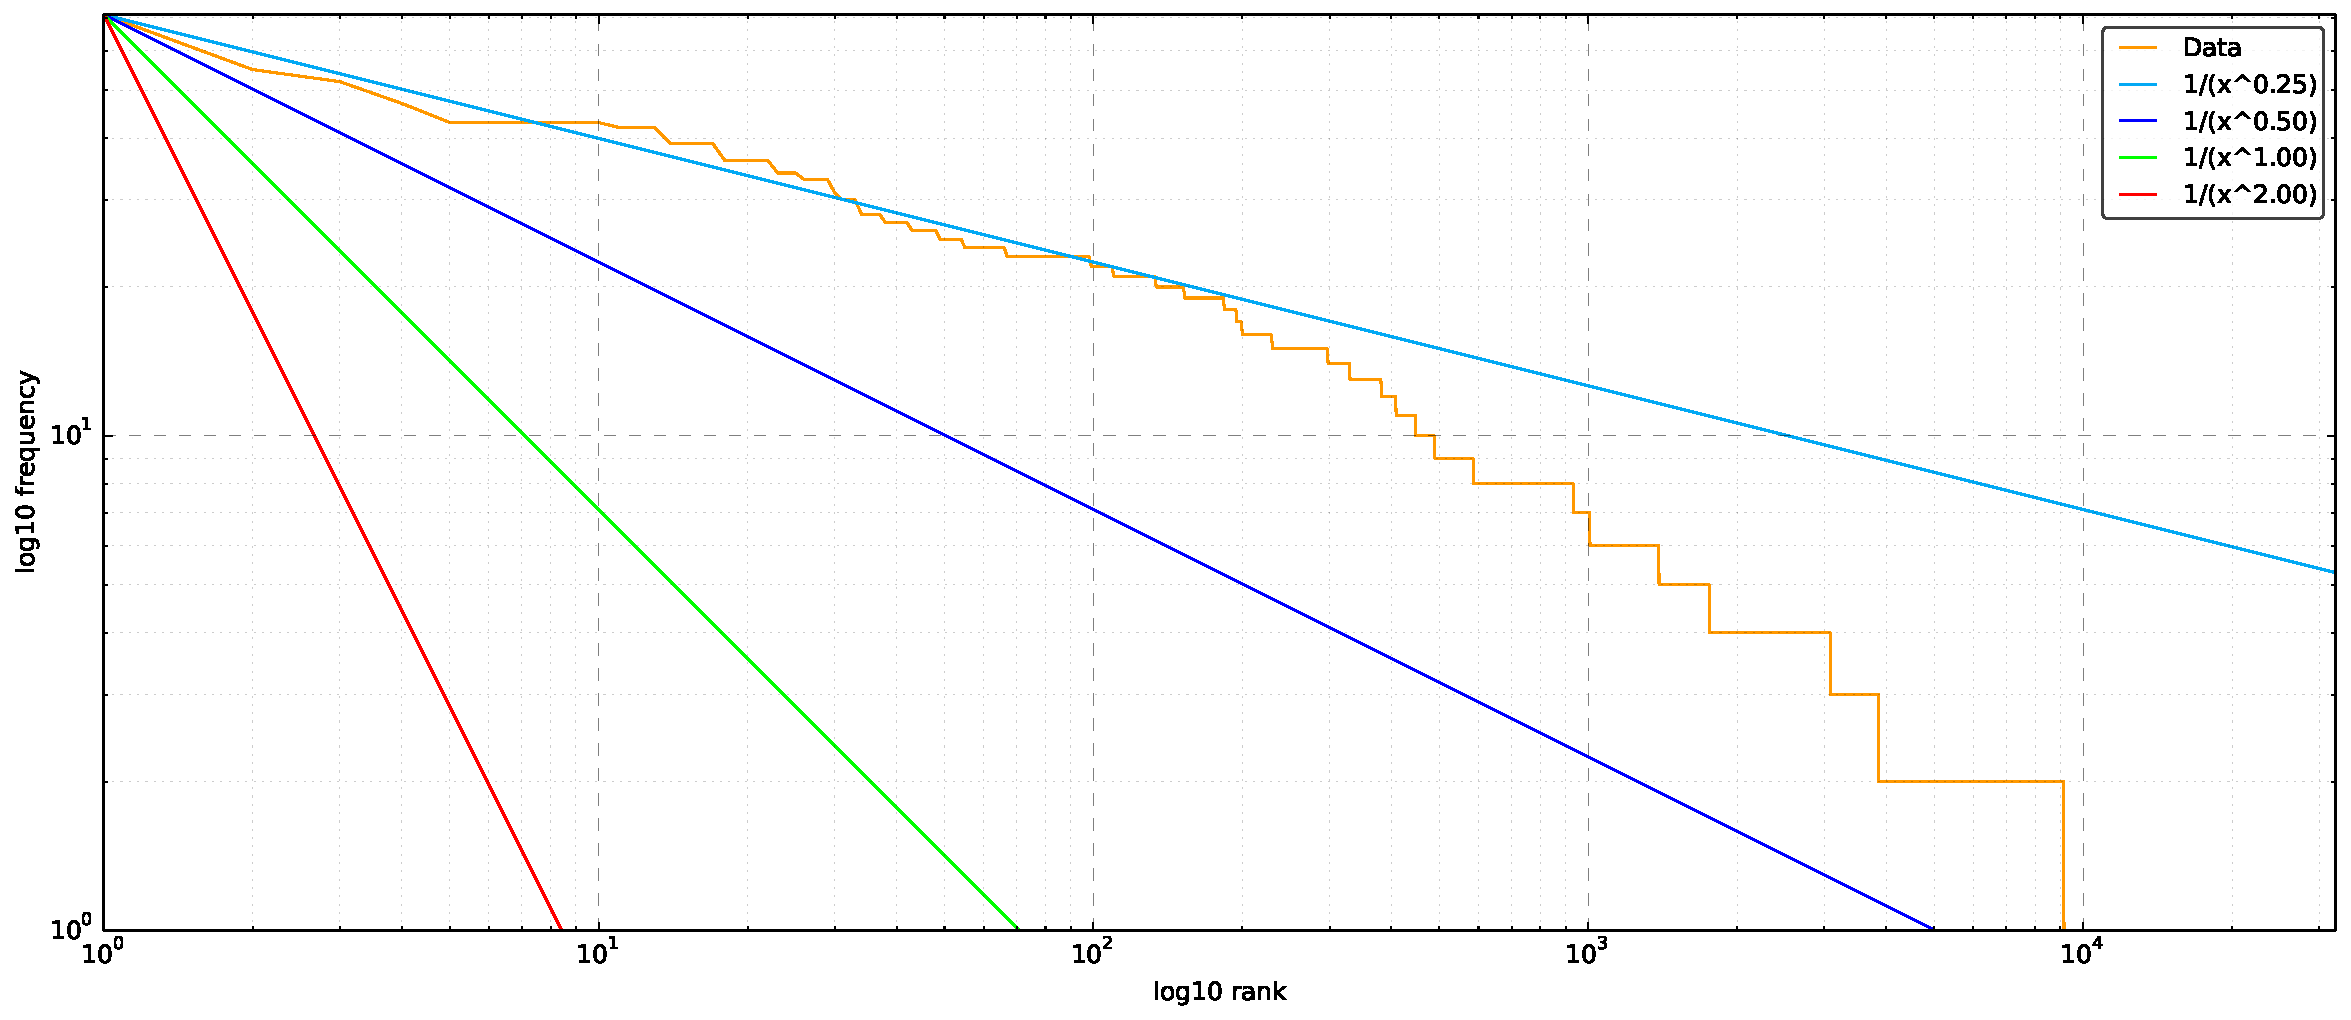
\includegraphics[width=0.9\linewidth]{figures/frequency-graphs/5-gram}
	\caption{Pentagram rank-frequency graph of tokenized dataset}
	\label{fig:rank-frequency-pentagram}
\end{figure}



\subsection{Most common and uncommon n-grams}

Analyzing the most common and uncommon words / n-grams is useful to gather a quick overview of the topics discussed in a given text corpus.

In \cref{tab:n-grams-counts} is shown the unique n-gram counts for the tokenized training dataset. It can be seen that the training dataset vocabulary is composed of 2487 unique words that were used to form 14140 unique bigrams, 8997 unique trigrams, 9306 unique tetragrams and 9138 unique pentagrams.

Looking at \cref{tab:most-common-unigrams,tab:least-common-unigrams} it can be seen that the most common unigrams present in the tokenized training dataset are mainly word articles, prepositions, conjunctions, punctuation and also the beginning and end of sentence tags (<s> and </s>) while the less common unigrams are mainly verbs, nouns and adjectives. Analyzing the \crefrange{tab:most-common-bigrams}{tab:least-common-pentagrams} we can see that the word variety and complexity increases as we move from bigrams to pentagrams.


\begin{table}[t]
	\caption{Total count of unique n-grams in the tokenized training dataset}
	\extrarowsep = 0.47ex
	\centering
	\begin{tabu} to 0.18\textwidth { X[l,m] X[r,m] }
		\rowfont{\bfseries\itshape} N-gram & Count \\
		\hline
		Unigram		&	 2487	\\
		Bigram		&	14140	\\
		Trigram		&	 8997	\\
		Tetragram	&	 9306	\\
		Pentagram	& 	 9138	\\
	\end{tabu}
	\label{tab:n-grams-counts}
\end{table}



\begin{table}[ht]
	\extrarowsep = 0.47ex
	\centering
	\begin{minipage}[t]{.35\linewidth}
		\caption{Most common unigrams}
		\begin{tabu} { X[2.0,l,m] X[r,m] }
			\rowfont{\bfseries\itshape} Unigram & Count \\
			\hline
			the		&	3692 \\
			.		&	3276 \\
			)		&	1745 \\
			(		&	1735 \\
			,		&	1433 \\
			</s> 	&	1357 \\
			<s>		&	1357 \\
			of		&	1235 \\
			to		&	1098 \\
			and		&	1032 \\
		\end{tabu}
		\label{tab:most-common-unigrams}
	\end{minipage}
	\hspace{2em}
	\begin{minipage}[t]{.35\linewidth}
		\caption{Least common unigrams}
		\begin{tabu} { X[2.0,l,m] X[r,m] }
			\rowfont{\bfseries\itshape} Unigram & Count \\
			\hline
			connected		&	1 \\
			disassembled	&	1 \\
			extend			&	1 \\
			fixed			&	1 \\
			heavy			&	1 \\
			motors			&	1 \\
			path			&	1 \\
			ridges			&	1 \\
			tolerance		&	1 \\
			upwards			&	1 \\
		\end{tabu}
		\label{tab:least-common-unigrams}
	\end{minipage}
\end{table}


\begin{table}[ht]
	\extrarowsep = 0.47ex
	\centering
	\begin{minipage}[t]{.4\linewidth}
		\caption{Most common bigrams}
		\begin{tabu} { X[2.5,l,m] X[r,m] }
			\rowfont{\bfseries\itshape} Bigram & Count \\
			\hline
			. </s>			&	1120 \\
			of the			&	 528 \\
			( \#			&	 523 \\
			( item			&	 481 \\
			<s> install		&	 270 \\
			main housing	&	 251 \\
			input shaft		&	 248 \\
			) .				&	 244 \\
			in the			&	 236 \\
			from the		&	 234 \\
		\end{tabu}
		\label{tab:most-common-bigrams}
	\end{minipage}
	\hspace{1em}
	\begin{minipage}[t]{.4\linewidth}
		\caption{Least common bigrams}
		\begin{tabu} { X[2.5,l,m] X[r,m] }
			\rowfont{\bfseries\itshape} Bigram & Count \\
			\hline
			engine assembly		&	1 \\
			leads to			&	1 \\
			minor adjustments	&	1 \\
			next step			&	1 \\
			open the			&	1 \\
			put lower			&	1 \\
			rotate it			&	1 \\
			sliding out			&	1 \\
			top gear			&	1 \\
			with care			&	1 \\
		\end{tabu}
		\label{tab:least-common-bigrams}
	\end{minipage}
\end{table}


\begin{table}[ht]
	\extrarowsep = 0.47ex
	\centering
	\begin{minipage}[t]{.45\linewidth}
		\caption{Most common trigrams}
		\begin{tabu} { X[2.5,l,m] X[r,m] }
			\rowfont{\bfseries\itshape} Trigram & Count \\
			\hline
			\& cone )			&	182 \\
			cup \& cone			&	182 \\
			) . </s>			&	146 \\
			pre - load			&	134 \\
			bearing pre -		&	118 \\
			bearing cone (		&	117 \\
			bearing cup (		&	106 \\
			end of the			&	102 \\
			into main housing	&	 97 \\
			main housing (		&	 89 \\
		\end{tabu}
		\label{tab:most-common-trigrams}
	\end{minipage}
	\hspace{0.5em}
	\begin{minipage}[t]{.45\linewidth}
		\caption{Least common trigrams}
		\begin{tabu} { X[2.5,l,m] X[r,m] }
			\rowfont{\bfseries\itshape} Trigram & Count \\
			\hline
			attach the piston		&	1 \\
			cutting the wires		&	1 \\
			electrical contact is	&	1 \\
			fold the conductor		&	1 \\
			install output shafts	&	1 \\
			proper function of		&	1 \\
			to the airframe			&	1 \\
			using the piston		&	1 \\
			with three screws		&	1 \\
			you push the			&	1 \\
		\end{tabu}
		\label{tab:least-common-trigrams}
	\end{minipage}
\end{table}


\begin{table}[ht]
	\extrarowsep = 0.47ex
	\centering
	\begin{minipage}[t]{.495\linewidth}
		\caption{Most common tetragrams}
		\begin{tabu} { X[4,l,m] X[r,m] }
			\rowfont{\bfseries\itshape} Tetragram & Count \\
			\hline
			cup \& cone )				&	182 \\
			bearing pre - load			&	118 \\
			bearing cone ( \#			&	 77 \\
			\& cone ) into				&	 71 \\
			bearing cup ( \#			&	 63 \\
			light coat of grease		&	 63 \\
			with light coat of			&	 55 \\
			pounds of rolling torque	&	 53 \\
			check bearing pre -			&	 52 \\
			main housing from the		&	 50 \\
		\end{tabu}
		\label{tab:most-common-tetragrams}
	\end{minipage}
	\begin{minipage}[t]{.495\linewidth}
		\caption{Least common tetragrams}
		\begin{tabu} { X[4,l,m] X[r,m] }
			\rowfont{\bfseries\itshape} Tetragram & Count \\
			\hline
			center the shaft on			&	1 \\
			connect the wire to			&	1 \\
			cutting the wires to		&	1 \\
			during the attachment of	&	1 \\
			lubricate the cam shaft		&	1 \\
			mount from the side			&	1 \\
			rod in the slot				&	1 \\
			together to make the		&	1 \\
			using the piston rod		&	1 \\
			you slide it into			&	1 \\
		\end{tabu}
		\label{tab:least-common-tetragrams}
	\end{minipage}
\end{table}


\begin{table}[ht]
	\extrarowsep = 0.47ex
	\centering
	\begin{minipage}[t]{.495\linewidth}
		\caption{Most common pentagrams}
		\begin{tabu} { X[4,l,m] X[r,m] }
			\rowfont{\bfseries\itshape} Pentagram & Count \\
			\hline
			cup \& cone ) into			&	71 \\
			with light coat of grease	&	55 \\
			check bearing pre - load	&	52 \\
			14 " to 16 "				&	47 \\
			" pounds of rolling torque	&	43 \\
			" to 16 " pounds			&	43 \\
			/ 2 to 1 hour				&	43 \\
			1 / 2 to 1					&	43 \\
			16 " pounds of rolling		&	43 \\
			to 16 " pounds of			&	43 \\
		\end{tabu}
		\label{tab:most-common-pentagrams}
	\end{minipage}
	\begin{minipage}[t]{.495\linewidth}
		\caption{Least common pentagrams}
		\begin{tabu} { X[5,l,m] X[1.25,r,m] }
			\rowfont{\bfseries\itshape} Pentagram & Count \\
			\hline
			area on shaft where seal		&	1 \\
			connect the wire to terminal	&	1 \\
			during the assembly process .	&	1 \\
			facing away from the exhaust	&	1 \\
			it is installed with two		&	1 \\
			lined up with each other		&	1 \\
			put shaft and install the		&	1 \\
			two steam inlets facing each	&	1 \\
			where it fits into the			&	1 \\
			with a screw driver ,			&	1 \\
		\end{tabu}
		\label{tab:least-common-pentagrams}
	\end{minipage}
\end{table}



\subsection{N-grams models smoothing}

Maximum likelihood estimation gives zero probability to word sequences that have not occurred in the training data. As such, it is necessary to redistribute some of the probability mass in order to ensure that there are no n-grams with the known vocabulary that have zero probability. This redistribution of probability mass is known as smoothing, because the resulting language model has smoother transitions in the n-gram probabilities.

One of the simplest smoothing techniques is the Laplace smoothing, which adds $\alpha$ (typically $\alpha=1$) to the n-gram counts. However, techniques such as the Witten Bell and Knesser Ney can achieve much better results (as can be seen in the much lower perplexity values shown in \cref{tab:n-grams-models-perplexities}).



\subsection{N-grams interpolation and backoff}

FF.



\subsection{Sentence generation using n-gram models}

N-gram models can be used to perform sentence generation by picking a starting n-gram and successively appending the most probable word by taking into account the last $n-1$ added words.

In \crefrange{subsec:unigram-sentences}{subsec:pentagram-sentences} are shown sentences generated using n-gram models built using the tokenized training dataset.
Analyzing \cref{subsec:unigram-sentences} it can be seen that a unigram model is not suitable for sentence generation because it does not retain word relations (the sentences are not syntactically correct and there is no coherence of ideas). Bigram models provide some improvements over unigrams, such as local coherence (as can be seen in \cref{subsec:bigram-sentences}). However bigram models are not able to generate long meaningful sentences. Moving to higher order n-grams improves the overall sentence complexity and coherence, as can be seen by analyzing \crefrange{subsec:trigram-sentences}{subsec:pentagram-sentences}. However creating higher order n-grams models requires much more processing time and they may still not be able to build syntactically correct and meaningful sentences. As such, n-gram models should be integrated with lexicalized probabilistic context free grammars in order to ensure syntactically correct sentences while retaining the type of language discourse present in the training dataset.



\subsubsection{Sentences generated using an unigram model}\label{subsec:unigram-sentences}

\begin{itemize}
	\item <s> part bearing threaded 3 the hole link seals to correct threaded the instructions install in be </s>
\end{itemize}


\subsubsection{Sentences generated using a bigram model}\label{subsec:bigram-sentences}

\begin{itemize}
	\item <s> install shim from bottom of rolling torque then slide gear in the outside of the columns to 14 " lbs . slide it coat of housing from the camshaft in the permanent marker . </s>
	\item <s> slide shaft ( \# 00762521 ) into the shims will cause seal toward body of rectifier , and secure it ' t fit over each spark plug installation , rotating the columns along both side of grease or replaced with bearings and gear in place , check that must be ground to wings , 1 . leave it on it to 16 ) and thread the magnets as you add washers . sequentially tighten front bearing cup ( 53074 ) </s>
	\item <s> the engine is seated down into a light coat of white lithium grease before deciding gearbox housing assemblies </s>
	\item <s> gearbox with bearing cap down over the eccentric strap ( 9 ) on each piston rod . there are slid in housing ( \# 00758655 cup , this style gearbox is needed . the two halves and adjustment </s>
	\item <s> check bearing and bearing to make sure it , and use the ends flush , coat of shaft has been assembled correct bearing pre - 80 x 1 hour . do not necessary . backlash is against snap ring on top of each of the threaded and the spark plug ( \# 00755628 cup try to the hub . ( item 39 ) onto lower bearings , either solvent . slide a 0 - 17 . if one piston rod and into main housing ( \# 00762522 ) , metal shop equipment . </s>
	\item <s> 2 - load . in horizontal hub on the three screws to the wire through input shaft ( item 3 nuts at this has been done fill with hammer and into main housing or further away from you near outer retaining screws farthest away from the rotor shaft gear till it seats against bearing spacer . install side bearing cup \& fourth , bearings \& cone ( fig . </s>
	\item <s> 3 ) , then nut above end of the distance from housing . </s>
	\item <s> when the ring ( 7 . 017 " to the spindle rod between blade shaft . recheck oil , gears ( 14 ) , they are against bearing cup \& cone is between each slot of the correct install output shaft with four ( \# 00760889 ) and components . 12 ) into main housing . using sealer at the head stud seals slide bearing adjusting nut ( \# 00758650 cup \& # 00748526 ) and further adjustment </s>
	\item <s> tighten bolts in place a 0 - 56 x 1 hour check stator core . , replace it is built and position and gently pry stator inside of the detent notches in the flywheel with light coat of rolling torque then slide shaft ) on each end of the alternator in the aerovee ' t fit mainshaft ( item 28 ) onto input seal ( \# 30 hex nut that require lapping as described in link ( 219 - lash between the chest on shims from bottom of the flanges of rolling torque . </s>
	\item <s> assembly ( item 17 . rotate the bottom out of this till input shaft , remove shims ( 53074 ) on the left . install output check the next assemblies into place of the panel for leaks , change the inside of the bearing pre - ring dgb - style ) finger tighten the female slide the passages . insert the process much more quickly as it . re - pounds of the inner bearing adjusting screw slotted bearing cup ( item 1 . </s>
\end{itemize}


\subsubsection{Sentences generated using a trigram model}\label{subsec:trigram-sentences}

\begin{itemize}
	\item <s> install output seal ( item 22 . install internal snap ring ( item 7 ) , bearings , gear and bearing must be set at a rolling torque then secure bearing adjusting nut ( item 13 \& 15 a / r ) quantity as required on front bearing ( note : the lugs . finger pressure . </s>
	\item <s> gearbox p / n 00769927 </s>
	\item <s> install input seal ( item 16 ) in each of the crankshaft , install all oil fill \& vent plugs and check for leaks , after set gear ( item 16 ) into inner bearing cup , lay a straight edge between the left half over the end of the stator is tight , file the slides unless otherwise specified , install shims against shims , file the small diameter of grease . using shims ( item 13 . </s>
	\item <s> 1 . install external clip on shaft . </s>
	\item <s> install the lower gear . </s>
	\item <s> 2 . drop input gear . </s>
	\item <s> 3 . apply an 18 ga . carefully inspect the hole in the cylinder mount . </s>
	\item <s> note : the bellcrank should be able to see through both holes that are the same time , install inner bearing cup . </s>
	\item <s> 4 . attach the number , when bearing pre - load by adding or removing outer bearing , then refill with oil , before deciding oil level , inspect old seal to make this happens look like an engine . </s>
	\item <s> when this task with the side of input shaft ( blade shaft gear and one outer cup , install output shaft bearing cone ( \# 00755613 ) . </s>
\end{itemize}


\subsubsection{Sentences generated using a tetragram model}\label{subsec:tetragram-sentences}

\begin{itemize}
	\item <s> gearbox p / n 00755697a </s>
	\item <s> install input shaft , shaft . insert output shaft with bearing cone on it up through main housing from the rear through rear bearing ( item 3 , from the front . slide shaft guiding it through input gear . slide shaft guiding leads do not touch the port face on each o - ring ( 40003 ) on each end of the valve spindle assembly ( a2004 ) through adjusting nuts that hold drive shaft ( item 1 ) install output shaft ( item 30 ) can drop through them up through indicator strap . position the bellcrank . after filing these screws flush , install shims ( \# 00755622 ) down over shaft till it seats against shoulder on shaft . install bearing cap down over input shaft . there may make sure that hold the guides . there may be one ore more used . </s>
	\item <s> install output shaft bearing , then take a few extra hole . install bearing cup ( item 13 \& 15 a / r ) and outer bearing cone . </s>
	\item <s> when this has no burrs that will will allow end play to regulator stud connector ( 219 - 1a ( \# 13 ) . once all is correct tighten till they are against input gear . install retaining snap ring retainer ( 51007 ) </s>
	\item <s> check bearing pre - load correct . in some cases it will be required to change the shims ( item 29 \& 3 ) 1 on output gear ( \# 00755506 ) on front of input shaft ( center shaft and ( item 8 ) do not put gear down into housing , this will prevent nut from turning and loosening up . </s>
	\item <s> tighten bearing adjusting nut till bearings have 14 " to 16 " pounds of rolling torque then secure bearing adjusting nut ( item 10 ) . </s>
	\item <s> install shims ( \# 00755619 ) in against bearing cup try to use the same amount of shims used it is seated against shim . insert the magnets . </s>
	\item <s> install the lower bearing cone ( \# 12b ) onto input shaft from the front till they are against the oil slinger . press the one nearest the middle of the crosshead end of the four ( 4 ) start to the base . tighten . </s>
	\item <s> install upper bearing cup . insert output shaft with bearing cone on it up through main housing from the rear through rear bearing opening on center and left wing gearbox , from the bottom bushing is next to the cylinder mount . </s>
	\item <s> install outer bearing cup ( item 12 cup \& cone ) ) down over output shaft . repeat steps 2 through both ends are very strong and after running 1 / 2 ” thicknesses together to get mixed up on " top of output shaft , the number of shims required will vary , try to put same amount of shims as were removed . install output gear ( \# 00758506 ) to 2 . 5 ” setscrew towards the arm of the bellcrank nearest you . rotate the crankshaft so one of main housing . slide lower output bearing ( 5 ) onto side shaft till it seats against the alternator . these are on the outside of the side drive gear in main housing ( \# 00762520 ) always install center input / output shaft ( \# 00755617 ) next to rear bearing ( item 3 ) down over input shaft , tighten nut ( item 10 ) onto top of output shaft , make sure that bearing is cleaned , drill a drop of oil on each eccentric where gear goes . install external clip ( 1 ) , make sure it is against against shims , install front input shaft bearing , then refill with oil , install top cover ( using sealer for gasket ) , oil plugs and check for leaks , after running mower 1 / 2 to 1 hour check oil level and recheck for leaks . </s>
\end{itemize}



\subsubsection{Sentences generated using a pentagram model}\label{subsec:pentagram-sentences}

\begin{itemize}
	\item <s> gearbox p / n 00757918 </s>
	\item <s> install output shaft ( blade shaft ) , shaft , bearings \& gear into main housing ( item 1 ) from the top , install lower bearing cup ( item 5 ) till it is seated into cup . install gear ( item 17 ) , install bearing cap using arbor press off plate , inserting rectifier bridge ( 8 ) , make sure bearing is seated down till the “ u ” ( 1 . 0mm ) into inside of main housing . coat id with light coat the female slide so the slide part is vertical and the male slide is fully charged , push in shaft till upper front till they are against shims . install rear seal ( item 11 ) . attach to 1 hour . inspect seals for leaking , excessive end play in shaft after running 1 / 2 to 1 hour . </s>
	\item <s> when this has been done fill gearbox with oil , before deciding gearbox is full . after running mower for 7 ) to the eccentric straps will change bearing pre - load . </s>
	\item <s> check bearing pre - load . output shaft should have no end play and bearing must be set at a rolling torque . </s>
	\item <s> tighten bearing adjusting nut above gear till bearings have a flat surface and slide the assembly over shaft and against upper id of seals with light coat of grease . </s>
	\item <s> install input shaft , shaft , bearings \& gear in main housing ( \# 00752362 ) into the best looking end play but back lash is correct , if shaft has end play but back - lash is correct . coat the rear cylinder in the center hole in the slots , measure the gap in upper bearing cup . </s>
	\item <s> install the lower bearing cone ( item 4 bearing spacer from the bottom . </s>
	\item <s> install upper bearing cup ( \# 00758655 cup \& cone ) over shaft from you . rotate the mount so they are vertical with the numbers will result . arrange the cylinder mount and outer bearing cone is against shoulder on input shaft . </s>
	\item <s> install input shaft ( pto ) from inside surface thinly with mineral spirits . when the switch is " back lash ) if bearing pre - load is right case . install it into housing . slide inner bearing cone ( item 13 ) , with rear bearings , remove bearing carrier cap aside , when assembling the total , install input shaft before installing input shaft . </s>
	\item <s> install rear input bearing cone ( \# 00755628 ) into lower housing from the bottom . put upper bearing cone ( item 4 . ( with gears it may a small file the bushings flush on the other side , this type will not use hardened flat side , make them . </s>
\end{itemize}



\subsection{N-gram models perplexity}

\begin{table}[t]
	\caption{Tokenized testing dataset overview}
	\extrarowsep = 0.47ex
	\centering
	\begin{tabu} to 0.33\textwidth { X[5,l,m] X[r,m] }
		\rowfont{\bfseries\itshape} Metric & Value \\
		\hline
		Sentences							&	   439	\\
		Words								&	 20829	\\
		Out of vocabulary words ignored		&	  4848	\\
		Zero probabilities words ignored	&	  1109	\\
	\end{tabu}
	\label{tab:n-grams-models-stats}
\end{table}


\begin{table}[t]
	\caption{N-grams models perplexities}
	\extrarowsep = 0.47ex
	\centering
	\begin{tabu} to 0.29\textwidth { X[2.5,l,m] X[r,m] }
		\rowfont{\bfseries\itshape} N-gram model & Perplexity \\
		\hline
		Unigram (no smoothing)		&	243.771		\\
		Unigram (Laplace add-1)		&	245.126		\\
		Unigram (Kneser-Ney)		&	243.771		\\
		Unigram (Witten-Bell)		&	245.126		\\
		Bigram (no smoothing)		&	164.299		\\
		Bigram (Laplace add-1)		&	182.235		\\
		Bigram (Kneser-Ney)			&	 56.408		\\
		Bigram (Witten-Bell)		&	 56.717		\\
		Trigram (no smoothing)		&	133.965		\\
		Trigram (Laplace add-1)		&	233.030		\\
		Trigram (Kneser-Ney)		&	 44.559		\\
		Trigram (Witten-Bell)		&	 45.160		\\
		Tetragram (no smoothing)	&	131.832		\\
		Tetragram (Laplace add-1)	&	245.794		\\
		Tetragram (Kneser-Ney)		&	 44.067		\\
		Tetragram (Witten-Bell)		&	 44.042		\\
		Pentagram (no smoothing)	&	132.059		\\
		Pentagram (Laplace add-1)	&	250.158		\\
		Pentagram (Kneser-Ney)		&	 45.725		\\
		Pentagram (Witten-Bell)		&	 44.281		\\
	\end{tabu}
	\label{tab:n-grams-models-perplexities}
\end{table}

\section{Conclusions}\label{sec:conclusions}

This paper presented the preparation and statistical analysis of a dataset for evaluating \gls{ner} systems targeted for industrial robotics applications. The dataset contains assembly operations of alternators, gearboxes and engines in textual form and is complemented with object pictures and assembly diagrams. For evaluating \gls{ner} systems using this dataset, each assembly operation has an associated list with the assembly objects and the quantities needed to successfully perform the product assembly. In order to have a representative dataset, it is provided assembly operations written in a professional and structured manner and also in an informal and colloquial language register. Moreover, it is given a brief statistical analysis of the dataset, with rank-frequency graphs, n-gram models perplexity and also some sentences generated using several n-gram models (from unigrams to pentagrams).

This dataset was built for evaluating \gls{ner} systems, but can also be used to evaluate information extraction and computer vision systems, given the large textual and image information that it provides for each assembly operation.

\section{Future work}\label{sec:future-work}

Future work for this dataset would include the tagging of all named entities in each assembly operation (instead of having a list for the entire procedure). Moreover, the assembly graph containing both the assembly order and the spatial disposition of the product components would be useful for validating more complex information extraction systems which intend to recover the full assembly knowledge from the text and image representation alone (without operator assistance).

For a system which aims to extract only the named entities in the assembly operations for speeding up object recognition (by restricting the database of object models to search for and recognize), it would be useful to start with the raw text from the \glspl{pdf} and perform an initial text preprocessing. This stage could include word tokenization, sentence splitting, \gls{pos} tagging and morphological analysis. Latter on, it could be used a gazetter in conjunction with machine learning algorithms (such as \glspl{hmm} or \glspl{crf}) to detect the named entities in the textual assembly operations. After having the named entities, it could be used an orthographic matcher to perform named entity coreference to find different mentions of the same entity and also type disambiguation in order to use word context to make sure that the semantic analysis was correct. The evaluation of a system with these goals can be done by comparing the list of named entities identified as assembly objects with the dataset validation list of product object components. Moreover, if the dataset has named entities tags for each word in the testing dataset, then a more complete evaluation can be done, allowing to assess the reliability of the entity disambiguation and coreference algorithms. Either way, this evaluation would result in the computation of the precision, recall, accuracy and F1 scores for the recognized entities given the list of entities that the \gls{ner} system was supposed to detect using a k-fold cross validation approach to split the dataset into training and test text.




%---------------------------------------------------------------------------------------------------
% Bibliography
%---------------------------------------------------------------------------------------------------

\bibliographystyle{IEEEtran}
\bibliography{references}


\end{document}
